%=========================================================================
% (c) 2014, 2015 Josef Lusticky

\chapter{Measurements}\label{chap:measurements}
The results presented in this thesis are based on the setup and basic settings described in chapter~\ref{chap:setup}.
The CentOS~7 operating system
was installed on the server with two Intel Xeon E5-2660 v3 CPUs
and Mellanox ConnectX-3 EN 40~Gbps Ethernet adapter, as described in section~\ref{sec:analysis-hardware}.
Each measurement put the server under 60~seconds of constant unidirectional traffic load,
as described in section~\ref{sec:analysis-metodology}.
Unless stated otherwise,
the bandwidth use is configured in frames per second with a unit of margin 50~000.

\section{CentOS~7 distribution kernel 3.10.0-123}
The CentOS~7 distribution kernel version 3.10.0-123.20.1.el7.x86\_64
was used in the measurements presented in this section.

	%=========================================================================
% (c) 2014, 2015 Josef Lusticky

% FINAL
\subsection{Measurement 1 - default configuration - single IPv4 flow}
The first measurement shows the routing performance with
IP addresses assigned, IP forwarding enabled and Netfilter rules flushed.

The IP addresses were assigned as described in section~\ref{sec:setup-server}.
The IP forwarding was enabled by echoing "1" to the /proc/sys/net/ipv4/ip\_forward file and the Netfilter rules
were flushed using {\it{iptables -F}}, because the default rules do not allow forwarding.
\\
\\
\begin{tabular}{ | l | l | l | l | }
\hline
Frame size & \% of link & bandwidth & frame rate \\
\hline
64     &  0.59\% & 0.24~Gb/s & 350~000 \\
594    &  4.30\% & 1.72~Gb/s & 350~000 \\
1518   & 10.77\% & 4.31~Gb/s & 350~000 \\
AMS-IX &  5.33\% & 2.13~Gb/s & 350~000 \\
\hline
\end{tabular}

	
	%=========================================================================
% (c) 2014, 2015 Josef Lusticky

% FINAL
\subsection{Measurement 2 - default configuration - 32 IPv4 flows}
Since the Linux kernel scaling mechanisms described in section~\ref{sec:linux-scaling}
are based on processing each flow by a different CPU,
the routing performance of the default configuration was tested against 32 IPv4 flows.
\\
\\
\begin{tabular}{ | l | l | l | l | }
\hline
Frame size & \% of link & bandwidth & frame rate \\
\hline
64     &  2.69\% &  1.08~Gb/s & 1~550~000 \\
594    & 19.65\% &  7.86~Gb/s & 1~600~000 \\
1518   & 49.22\% & 19.69~Gb/s & 1~650~000 \\
AMS-IX & 24.34\% &  9.74~Gb/s & 1~600~000 \\
\hline
\end{tabular}
\\
\\
As expected, the scaling mechanisms help to increase the routing performance of the Linux kernel.
The scaling mechanisms perform better when forwarding larger frames.
This may be caused by differences in memory management allocations,
since the memory management is common for all CPUs present in the system.

	
	%=========================================================================
% (c) 2014, 2015 Josef Lusticky

% FINAL
\subsection{Measurement 3 - single IPv4 flow}
Unlike the previous measurements,
the following measurements use the complete setup described in section~\ref{sec:setup-server} to increase the throughput.
\\
\\
\begin{tabular}{ | l | l | l | l | }
\hline
Frame size & \% of link & bandwidth & frame rate \\
\hline
64     &  1.68\% &  0.67~Gb/s & 1~000~000 \\
594    & 12.28\% &  4.91~Gb/s & 1~000~000 \\
1518   & 30.76\% & 12.30~Gb/s & 1~000~000 \\
AMS-IX & 15.22\% &  6.09~Gb/s & 1~000~000 \\
\hline
\end{tabular}
\\
\\
The Linux kernel is able to forward 1~million IPv4 packets per second on a single core.
\\
The following partial output of the /proc/interrupts file shows the interrupt mapping:
\begin{lstlisting}
      ... CPU8  CPU9   CPU10 CPU11 CPU12  ...
178:  ...    0     0  255725     0     0  ...  enp129s0-0
179:  ...    0     0       0     0     0  ...  enp129s0-1
180:  ...    0     0       0     0     0  ...  enp129s0-2
181:  ...    0     0       0     0     0  ...  enp129s0-3
182:  ...    0     0       0     0     0  ...  enp129s0-4
183:  ...    0     0       0     0     0  ...  enp129s0-5
184:  ...    0     0       0     0     0  ...  enp129s0-6
185:  ...    0     0       0     0     0  ...  enp129s0-7
186:  ...    0     0       0     0     0  ...  enp129s0d1-0
187:  ...    0     0       0     0     0  ...  enp129s0d1-1
188:  ...    0     0       0     0     0  ...  enp129s0d1-2
189:  ...    0     0       0     0     0  ...  enp129s0d1-3
190:  ...    0     0       0     0     0  ...  enp129s0d1-4
191:  ...    0     0  313670     0     0  ...  enp129s0d1-5
192:  ...    0     0       0     0     0  ...  enp129s0d1-6
193:  ...    0     0       0     0     0  ...  enp129s0d1-7
\end{lstlisting}
All packets are assigned to a single queue, in this case the queue number 5 ({\it{enp129s0d1}} is the receiving interface).
The smp\_affinity files show that the Linux kernel
automatically assigned each interrupt to the CPUs 10-19 and 30-39.
\begin{lstlisting}
cat /proc/irq/178/smp_affinity_list
	10-19,30-39
cat /proc/irq/179/smp_affinity_list
	10-19,30-39
...
cat /proc/irq/193/smp_affinity_list
	10-19,30-39
\end{lstlisting}
The {\it{lscpu}} utility or the Intel Performance Counter Monitor can be used to
verify that the CPUs 10-19 and 30-39 are logical cores of the CPU in Socket 1.
The CPU in this socket is directly connected to the PCI-Express link, as shown in figure~\ref{fig:setup-supermicro-board}.
\\
\\
The {\it{perf}} utility can be used to list the functions utilising the CPU 10.
\begin{lstlisting}
perf top -C 10
  11.42%  [kernel]  [k] fib_table_lookup
   9.62%  [kernel]  [k] _raw_spin_lock
   6.65%  [kernel]  [k] mlx4_en_xmit
   4.84%  [kernel]  [k] memcpy
   4.03%  [kernel]  [k] mlx4_en_complete_rx_desc
   3.61%  [kernel]  [k] check_leaf.isra.7
   3.52%  [kernel]  [k] mlx4_en_free_tx_desc.isra.22
   3.42%  [kernel]  [k] mlx4_en_process_rx_cq
   3.16%  [kernel]  [k] mlx4_en_poll_tx_cq
   2.89%  [kernel]  [k] put_compound_page
   2.72%  [kernel]  [k] dev_queue_xmit
\end{lstlisting}
The kernel spends most of the time on FIB lookup, which is performed by the {\it{fib\_table\_lookup}} function described
in section~\ref{sec:linux-routing}, and on locking.
\\
\\
The following listing shows the cache utilisation on all CPUs present in the system.
\begin{lstlisting}[language=TeX]
 L3MISS: L3 cache misses
 L2MISS: L2 cache misses (including other core's L2 cache *hits*)
 L3HIT : L3 cache hit ratio (0.00-1.00)
 L2HIT : L2 cache hit ratio (0.00-1.00)
 L3CLK : ratio of CPU cycles lost due to L3 cache misses (0.00-1.00), in some cases could be >1.0 due to a higher memory latency
 L2CLK : ratio of CPU cycles lost due to missing L2 cache but still hitting  L3 cache (0.00-1.00)
 L3OCC : L3 occupancy (in KBytes)

 Core (SKT) | L3MISS | L2MISS | L3HIT | L2HIT | L3CLK | L2CLK |  L3OCC

   0    0     4052       23 K    0.83    0.26    0.19    0.18      120
   1    0       52     1542      0.97    0.14    0.03    0.17       80
   2    0       37     1458      0.97    0.14    0.02    0.17      200
   3    0       42     1489      0.97    0.14    0.02    0.13        0
   4    0       36     1460      0.98    0.15    0.02    0.16        0
   5    0      223     1695      0.87    0.22    0.00    0.00       80
   6    0        4      542      0.99    0.13    0.00    0.12       40
   7    0        4      539      0.99    0.12    0.00    0.12        0
   8    0        4      533      0.99    0.12    0.00    0.11        0
   9    0       20      589      0.97    0.10    0.02    0.11       40
  10    1     1179     2608 K    1.00    0.88    0.00    0.04      240
  11    1      129      586      0.78    0.11    0.16    0.13        0
  12    1        7      531      0.99    0.12    0.01    0.16        0
  13    1      446     2223      0.80    0.14    0.06    0.05       80
  14    1        7      531      0.99    0.14    0.01    0.12        0
  15    1        7      535      0.99    0.13    0.01    0.13        0
  16    1        6      534      0.99    0.13    0.01    0.12        0
  17    1       16      675      0.98    0.17    0.01    0.12        0
  18    1       10      534      0.98    0.13    0.01    0.12        0
  19    1       24      607      0.96    0.11    0.02    0.10        0
  20    0      175     1090      0.84    0.07    0.08    0.14        0
  21    0        9      598      0.98    0.13    0.01    0.18        0
  22    0       80      974      0.92    0.14    0.01    0.03        0
  23    0       10      583      0.98    0.13    0.01    0.10        0
  24    0       15      831      0.98    0.12    0.01    0.17        0
  25    0       41      582      0.93    0.13    0.03    0.11        0
  26    0        4      513      0.99    0.13    0.00    0.13        0
  27    0        5      534      0.99    0.13    0.01    0.14       40
  28    0        5      534      0.99    0.12    0.01    0.12       40
  29    0       34      659      0.95    0.12    0.03    0.12        0
  30    1      102      603      0.83    0.12    0.16    0.17       40
  31    1       12      627      0.98    0.34    0.01    0.15      120
  32    1       37      544      0.93    0.12    0.05    0.16        0
  33    1       11      584      0.98    0.13    0.01    0.16       40
  34    1        7      528      0.99    0.14    0.01    0.17       40
  35    1        8      541      0.99    0.16    0.01    0.17        0
  36    1        8      541      0.99    0.12    0.01    0.16        0
  37    1       11      541      0.98    0.13    0.02    0.17       40
  38    1       11      553      0.98    0.12    0.01    0.16        0
  39    1     2105     4296      0.51    0.65    0.13    0.03      480
-------------------------------------------------------------------------
 SKT    0     4852       40 K    0.88    0.21    0.03    0.05      640
 SKT    1     4143     2624 K    1.00    0.87    0.00    0.04     1080
-------------------------------------------------------------------------
 TOTAL  *     8995     2664 K    1.00    0.87    0.00    0.04      N/A
\end{lstlisting}
The CPU 10 is performing the work related to TCP/IP processing.
Most of the cache misses are L2 miss, but there are also L3 misses.
The number of L3 misses is greatly reduced by the Intel Data Direct I/O technology,
as described in section~\ref{sec:analysis-hardware}.
The L2 hit ratio is 88\%, while L3 hit ration is almost 100\%.
Other CPUs are in idle state, except for CPU~0, which is running the Intel PCM and prints the output.

	
	%=========================================================================
% (c) 2014, 2015 Josef Lusticky

% FINAL
\subsection{Measurement 4 - 32 independent IPv4 flows}
This measurement can be compared with Measurement~2, except that the {\it{irqbalance}} daemon is disabled.
Therefore, the IRQ mapping is left untouched in its default state.
\\
\\
\begin{tabular}{ | l | l | l | l | }
\hline
Frame size & \% of link & bandwidth & frame rate \\
\hline
64     &  1.26\% &  0.50~Gb/s & 750~000 \\
594    & 12.28\% &  4.91~Gb/s & 800~000 \\
1518   & 24.61\% &  9.84~Gb/s & 800~000 \\
AMS-IX & 15.22\% &  6.09~Gb/s & 800~000 \\
\hline
\end{tabular}
\\
\\
When forwarding IP packets from multiple IPv4 flows on a single CPU,
the routing performance of the Linux kernel drops by 20\% against forwarding a single IPv4 flow.
The following listing shows that
the packets are uniformly distributed among all hardware queues.
However, the interrupts are not distributed among CPUs.
\begin{lstlisting}
      ... CPU8  CPU9   CPU10 CPU11 CPU12  ...
178:  ...    0     0  474701     0     0  ...  enp129s0-0
179:  ...    0     0       0     0     0  ...  enp129s0-1
180:  ...    0     0       0     0     0  ...  enp129s0-2
181:  ...    0     0       0     0     0  ...  enp129s0-3
182:  ...    0     0       0     0     0  ...  enp129s0-4
183:  ...    0     0       0     0     0  ...  enp129s0-5
184:  ...    0     0       0     0     0  ...  enp129s0-6
185:  ...    0     0       0     0     0  ...  enp129s0-7
186:  ...    0     0  317322     0     0  ...  enp129s0d1-0
187:  ...    0     0  317648     0     0  ...  enp129s0d1-1
188:  ...    0     0  317231     0     0  ...  enp129s0d1-2
189:  ...    0     0  317384     0     0  ...  enp129s0d1-3
190:  ...    0     0  317114     0     0  ...  enp129s0d1-4
191:  ...    0     0  317291     0     0  ...  enp129s0d1-5
192:  ...    0     0  317190     0     0  ...  enp129s0d1-6
193:  ...    0     0  317964     0     0  ...  enp129s0d1-7
\end{lstlisting}
Each receive queue triggers roughly the same number of interrupts as in the previous measurement,
but overall the NIC triggers much more interrupts.
The kernel spends more time on running the interrupt service routine code.
Apart from servicing interrupts, the kernel must fetch the packets from different ingress queues,
which in turn may need additional locking.
\\
The following listing shows partial output of {\it{perf}}:
\begin{lstlisting}
perf top -C 10
  12.07%  [kernel]  [k] _raw_spin_lock
   8.68%  [kernel]  [k] fib_table_lookup
   5.01%  [kernel]  [k] mlx4_en_xmit
   4.63%  [kernel]  [k] mlx4_en_process_rx_cq
   3.64%  [kernel]  [k] __netif_receive_skb_core
   3.49%  [kernel]  [k] memcpy
   3.08%  [kernel]  [k] irq_entries_start
   2.68%  [kernel]  [k] mlx4_eq_int
   2.33%  [kernel]  [k] mlx4_en_poll_tx_cq
   2.24%  [kernel]  [k] ip_route_input_noref
\end{lstlisting}
The kernel spends most of the time on locking and FIB table lookup.

	
	%=========================================================================
% (c) 2014, 2015 Josef Lusticky

% FINAL
\subsection{Measurement 5 - single IPv4 flow over QPI}
Instruct the kernel to use the CPU~9 for processing the RX interrupts.
The softirq and forwarding code runs on CPU~9.
\begin{lstlisting}[language=TeX]
for i in `seq 178 193` ; do echo 9 > /proc/irq/\$i/smp_affinity_list ;done
\end{lstlisting}
The CPU~9 is not directly connected to the PCI-Express link with the NIC,
so QPI links between CPUs are used.

\begin{tabular}{ | l | l | l | l | }
\hline
Frame size & \% of link & bandwidth & frame rate \\
\hline
64     &  1.09\% &  0.44~Gb/s & 650~000 \\
594    &  7.98\% &  3.19~Gb/s & 650~000 \\
1518   & 19.99\% &  8.00~Gb/s & 650~000 \\
AMS-IX &  9.89\% &  3.96~Gb/s & 650~000 \\
\hline
\end{tabular}
The routing perfomance drops by 35\% when it is performed by
a CPU not directly connected to the PCI-Express link with the NIC.

\begin{lstlisting}[language=TeX]
 L3MISS: L3 cache misses
 L2MISS: L2 cache misses (including other core's L2 cache *hits*)
 L3HIT : L3 cache hit ratio (0.00-1.00)
 L2HIT : L2 cache hit ratio (0.00-1.00)
 L3CLK : ratio of CPU cycles lost due to L3 cache misses (0.00-1.00), in some cases could be >1.0 due to a higher memory latency
 L2CLK : ratio of CPU cycles lost due to missing L2 cache but still hitting  L3 cache (0.00-1.00)
 L3OCC : L3 occupancy (in KBytes)


 Core (SKT) | L3MISS | L2MISS | L3HIT | L2HIT | L3CLK | L2CLK |  L3OCC

   0    0     6209       24 K    0.75    0.32    0.19    0.12      480
   1    0       13      546      0.98    0.12    0.01    0.14      640
   2    0      154     4746      0.97    0.16    0.03    0.18       40
   3    0       16     1452      0.99    0.14    0.01    0.15        0
   4    0       68     1164      0.94    0.25    0.00    0.00       80
   5    0       10      537      0.98    0.13    0.01    0.14      160
   6    0        5      538      0.99    0.13    0.01    0.14        0
   7    0       10      543      0.98    0.12    0.01    0.13        0
   8    0       10      548      0.98    0.11    0.01    0.11        0
   9    0     2002 K   2798 K    0.28    0.74    0.20    0.02     2360
  10    1      790       12 K    0.94    0.14    0.08    0.24     4640
  11    1       29      985      0.97    0.12    0.02    0.15        0
  12    1       22      569      0.96    0.11    0.02    0.09        0
  13    1      325     2112      0.85    0.15    0.05    0.06       40
  14    1      238     1328      0.82    0.16    0.05    0.05      120
  15    1       28      526      0.95    0.16    0.02    0.07       40
  16    1       32      572      0.94    0.13    0.02    0.07        0
  17    1       27      563      0.95    0.11    0.02    0.08        0
  18    1       20      563      0.96    0.12    0.01    0.09       40
  19    1       30      606      0.95    0.11    0.02    0.09       40
  20    0      158     1017      0.84    0.07    0.08    0.13       40
  21    0       10      553      0.98    0.13    0.02    0.20        0
  22    0       10      739      0.99    0.10    0.01    0.16       40
  23    0        7      574      0.99    0.13    0.01    0.18        0
  24    0       10      578      0.98    0.14    0.01    0.16        0
  25    0        4      535      0.99    0.14    0.01    0.16        0
  26    0       11      551      0.98    0.12    0.01    0.16        0
  27    0       11      550      0.98    0.13    0.01    0.13        0
  28    0       10      560      0.98    0.13    0.01    0.14        0
  29    0       97     5729      0.98    0.07    0.00    0.05        0
  30    1      185      911      0.80    0.08    0.10    0.12        0
  31    1       19      572      0.97    0.11    0.02    0.13        0
  32    1       15      556      0.97    0.13    0.02    0.13       80
  33    1       23      591      0.96    0.13    0.02    0.12       40
  34    1       21      555      0.96    0.12    0.01    0.09        0
  35    1       21      539      0.96    0.15    0.02    0.09      120
  36    1       23      555      0.96    0.13    0.02    0.09        0
  37    1       63      684      0.91    0.18    0.01    0.02        0
  38    1       16      555      0.97    0.14    0.01    0.10        0
  39    1     4826     7108      0.32    0.52    0.24    0.02        0
------------------------------------------------------------------------
 SKT    0     2009 K   2844 K    0.29    0.73    0.20    0.02     3840
 SKT    1     6753       32 K    0.79    0.26    0.10    0.08     5160
------------------------------------------------------------------------
 TOTAL  *     2015 K   2877 K    0.30    0.73    0.19    0.02      N/A
\end{lstlisting}

CPU~9 performs the actual forwarding, while CPU~10
is busy with the QPI communication overhead.

\begin{lstlisting}
Intel(r) QPI data traffic estimation in bytes (data traffic coming to CPU/socket through QPI links):

               QPI0     QPI1    |  QPI0   QPI1  
----------------------------------------------------------------------------------------------
 SKT    0       90 M     90 M   |    0%     0%   
 SKT    1       70 M     71 M   |    0%     0%   
----------------------------------------------------------------------------------------------
Total QPI incoming data traffic:  323 M     QPI data traffic/Memory controller traffic: 0.39
\end{lstlisting}
Both QPI links are used.


perf top -C 9
\begin{lstlisting}
  21.25%  [kernel]  [k] _raw_spin_lock
  11.61%  [kernel]  [k] memcpy
   6.69%  [kernel]  [k] fib_table_lookup
   6.60%  [kernel]  [k] skb_gro_reset_offset
   4.55%  [kernel]  [k] udp_gro_receive
   3.96%  [kernel]  [k] mlx4_en_xmit
   3.44%  [kernel]  [k] mlx4_en_process_rx_cq
   2.93%  [kernel]  [k] mlx4_en_poll_tx_cq
\end{lstlisting}

perf top -C 10
\begin{lstlisting}
   9.77%  [kernel]  [k] find_busiest_group
   3.47%  [kernel]  [k] cpumask_next_and
   3.01%  [kernel]  [k] _raw_spin_lock
   2.93%  [kernel]  [k] ktime_get
   2.59%  [kernel]  [k] mlx4_en_DUMP_ETH_STATS
   2.58%  [kernel]  [k] run_timer_softirq
   2.36%  [kernel]  [k] idle_cpu
   2.22%  [kernel]  [k] __schedule
\end{lstlisting}

	
	%=========================================================================
% (c) 2014, 2015 Josef Lusticky

% FINAL
\subsection{Measurement 6 - 32 IPv4 flows with irqbalance daemon}
The measurement includes the {\it{irqbalance}} daemon enabled.
The {\it{irqbalance}} daemon is responsible for dynamically assigning the interrupts to CPUs
using the files found under /proc/irq/{\it{NUMBER}}/smp\_affinity,
as described in subsection~\ref{sub:analysis-settings-procfs}.
\\
\\
\begin{tabular}{ | l | l | l | l | }
\hline
Frame size & \% of link & bandwidth & frame rate \\
\hline
64     &  8.99\% &  3.60~Gb/s & 5~350~000 \\
594    & 68.15\% & 27.26~Gb/s & 5~550~000 \\
1518   & 98.50\% & 39.40~Gb/s & 3~202~210 \\
AMS-IX & 88.25\% & 35.30~Gb/s & 5~800~000 \\
\hline
\end{tabular}
\\
\\
The scaling mechanisms of the Linux kernel take advantage of interrupt assignment
done by the {\it{irqbalance}} daemon.
The server is able to route almost 36~Gbps of the simulated AMS-IX internet traffic.
The measurement further confirms that the scaling mechanisms are sensitive to the frame size.
The measurement featuring 1518~octet frames was configured to use 98.5\% of the link bandwidth.
\\
The following listing shows that the {\it{irqbalance}} daemon assigned IRQs to CPUs 11-18, 30 and 33-39.
The CPUs 12-19 are serving RX interrupts, while the CPUs 30-39 are serving TX interrupts
({\it{en29d1}} represents the receiving interface).

\newpage

\begin{landscape}
\vspace*{\fill}
\begin{lstlisting}
     CPU12 CPU13 CPU14 CPU15 CPU16 CPU17 CPU18 CPU19  CPU30  CPU33  CPU34  CPU35  CPU36  CPU37  CPU38  CPU39
178:     0     0     0     0     0     0     0     0      0 292448      0      0      0      0      0      0 en29-0
179:     0     0     0     0     0     0     0     0      0      0 292978      0      0      0      0      0 en29-1
180:     0     0     0     0     0     0     0     0      0      0      0 292698      0      0      0      0 en29-2
181:     0     0     0     0     0     0     0     0      0      0      0      0 286435      0      0      0 en29-3
182:     0     0     0     0     0     0     0     0      0      0      0      0      0 282449      0      0 en29-4
183:     0     0     0     0     0     0     0     0      0      0      0      0      0      0 288839      0 en29-5
184:     0     0     0     0     0     0     0     0      0      0      0      0      0      0      0 327901 en29-6
185:     0     0     0     0     0     0     0     0 325935      0      0      0      0      0      0      0 en29-7
186: 53145     0     0     0     0     0     0     0      0      0      0      0      0      0      0      0 en29d1-0
187:     0 53090     0     0     0     0     0     0      0      0      0      0      0      0      0      0 en29d1-1
188:     0     0 39978     0     0     0     0     0      0      0      0      0      0      0      0      0 en29d1-2
189:     0     0     0 40484     0     0     0     0      0      0      0      0      0      0      0      0 en29d1-3
190:     0     0     0     0 40072     0     0     0      0      0      0      0      0      0      0      0 en29d1-4
191:     0     0     0     0     0 39982     0     0      0      0      0      0      0      0      0      0 en29d1-5
192:     0     0     0     0     0     0 40488     0      0      0      0      0      0      0      0      0 en29d1-6
193:     0     0     0     0     0     0     0 43262      0      0      0      0      0      0      0      0 en29d1-6
\end{lstlisting}
\vspace*{\fill}
\end{landscape}

\noindent
\\
The listing bellow shows the cache use.
\begin{lstlisting}[language=TeX]
 L3MISS: L3 cache misses 
 L2MISS: L2 cache misses (including other core's L2 cache *hits*) 
 L3HIT : L3 cache hit ratio (0.00-1.00)
 L2HIT : L2 cache hit ratio (0.00-1.00)
 L3CLK : ratio of CPU cycles lost due to L3 cache misses (0.00-1.00), in some cases could be >1.0 due to a higher memory latency
 L2CLK : ratio of CPU cycles lost due to missing L2 cache but still hitting L3 cache (0.00-1.00)

 Core (SKT) | L3MISS | L2MISS | L3HIT | L2HIT | L3CLK | L2CLK |  L3OCC

   0    0     1076       11 K    0.91    0.17    0.01    0.01      120
   1    0      574     4139      0.86    0.12    0.10    0.14       40
   2    0      241     1421      0.83    0.18    0.12    0.12        0
   3    0      658       11 K    0.94    0.09    0.07    0.24        0
   4    0       19      580      0.97    0.14    0.02    0.12        0
   5    0       78      363      0.79    0.25    0.03    0.03        0
   6    0       65      710      0.91    0.15    0.04    0.10       40
   7    0       19      544      0.97    0.12    0.02    0.10       40
   8    0       13      648      0.98    0.11    0.01    0.08        0
   9    0       32      582      0.95    0.11    0.02    0.08        0
  10    1     1007     3598      0.72    0.06    0.72    0.37       40
  11    1     4452     3802 K    1.00    0.45    0.00    0.10       40
  12    1     4932     3770 K    1.00    0.42    0.00    0.10      240
  13    1     6273     4131 K    1.00    0.51    0.00    0.09       40
  14    1     5086     4211 K    1.00    0.52    0.00    0.09       80
  15    1     4762     4211 K    1.00    0.50    0.00    0.10       80
  16    1     4453     4111 K    1.00    0.54    0.00    0.09       80
  17    1     4680     4124 K    1.00    0.56    0.00    0.09      160
  18    1     4737     4275 K    1.00    0.48    0.00    0.10       80
  19    1      105      573      0.82    0.18    0.18    0.17        0
  20    0      170      979      0.83    0.06    0.07    0.10       40
  21    0       16      692      0.98    0.10    0.01    0.12        0
  22    0       12      570      0.98    0.12    0.01    0.13        0
  23    0       15      839      0.98    0.10    0.01    0.13        0
  24    0       13      532      0.98    0.16    0.02    0.14        0
  25    0       22      441      0.95    0.21    0.01    0.06        0
  26    0       14      540      0.97    0.14    0.02    0.13        0
  27    0        9      516      0.98    0.15    0.01    0.13        0
  28    0      268     2659      0.90    0.09    0.10    0.18       40
  29    0      239      916      0.74    0.15    0.10    0.06        0
  30    1     1238     2816 K    1.00    0.60    0.00    0.27      680
  31    1       54      560      0.90    0.25    0.09    0.19       80
  32    1     3416     9666      0.65    0.20    0.72    0.27       40
  33    1       14 K   3887 K    1.00    0.64    0.00    0.27      640
  34    1       16 K   3969 K    1.00    0.63    0.00    0.27      960
  35    1       15 K   3881 K    1.00    0.64    0.00    0.27      960
  36    1       14 K   3878 K    1.00    0.63    0.00    0.27      880
  37    1       14 K   3920 K    1.00    0.63    0.00    0.27      440
  38    1       17 K   4014 K    1.00    0.63    0.00    0.27      600
  39    1     2106     2853 K    1.00    0.60    0.00    0.28     1240
------------------------------------------------------------------------
 SKT    0     3553       41 K    0.91    0.13    0.01    0.03      320
 SKT    1      141 K     61 M    1.00    0.57    0.00    0.14     7360
------------------------------------------------------------------------
 TOTAL  *      144 K     61 M    1.00    0.57    0.00    0.14      N/A 
\end{lstlisting}
The measurement featuring 1518~octet frames is the first measurement saturating the 40~Gbps Ethernet connection.
Intel PCM can be used to monitor the PCI-Express utilisation:
\begin{lstlisting}
Skt | PCIe Rd (B) | PCIe Wr (B)
 0         5270 K          86 K
 1           11 G        5422 M
--------------------------------
 *           11 G        5422 M
\end{lstlisting}
The PCI-Express link could be saturated when forwarding bidirectional traffic
- the PCI-Express 3.0 x8 throughput is 7~876.8~MB/s as calculated in section~\ref{sec:40gbe-throughput}.
Note, that there seems to be a bug in Intel PCM related to displaying
the PCIe Read bandwidth - it always shows double the expected value (11~Gigabytes does not make sense).

	
	%=========================================================================
% (c) 2014, 2015 Josef Lusticky

% FINAL
\subsection{Measurement 7 - 32 IPv4 flows with manual IRQ affinity mappings}
While {\it{irqbalance}} mapped the interrupts inteligently, it is always worth checking the mappings.
The dynamic mappings made by the {\it{irqbalance}} daemon can change during the run-time, which may lead
to unpredictable perfomance drops.
\\
The following listing shows the interrupt mapping scheme used during this measurement.
Unlike the mapping assigned by the {\it{irqbalance}} daemon,
this mapping targets both RX and TX interrupts to 8 CPUs only.
Additionally, Transmission Packet Steering (XPS) mechanism was configured
to maps each exclusively to a single CPUs, as described in section~\ref{sec:linux-scaling}.
\begin{lstlisting}[language=TeX]
echo 1 > /proc/irq/default_smp_affinity     # mask for new registered irqs
echo 0 | tee /proc/irq/*/smp_affinity_list  # assign all IRQs to CPU 0

echo 18 > /proc/irq/177/smp_affinity_list   # assign mlx4-async IRQ to CPU 18

echo 10 > /proc/irq/178/smp_affinity_list   # enp129s0-0 IRQ to CPU 10
echo 11 > /proc/irq/179/smp_affinity_list
echo 12 > /proc/irq/180/smp_affinity_list
echo 13 > /proc/irq/181/smp_affinity_list
echo 14 > /proc/irq/182/smp_affinity_list
echo 15 > /proc/irq/183/smp_affinity_list
echo 16 > /proc/irq/184/smp_affinity_list
echo 17 > /proc/irq/185/smp_affinity_list   # enp192s0-7 IRQ to CPU 17

echo 10 > /proc/irq/186/smp_affinity_list   # enp192s0d1-0 IRQ to CPU 10
echo 11 > /proc/irq/187/smp_affinity_list
echo 12 > /proc/irq/188/smp_affinity_list
echo 13 > /proc/irq/189/smp_affinity_list
echo 14 > /proc/irq/190/smp_affinity_list
echo 15 > /proc/irq/191/smp_affinity_list
echo 16 > /proc/irq/192/smp_affinity_list
echo 17 > /proc/irq/193/smp_affinity_list   # enp192s0d1-7 IRQ to CPU 17

# clear XPS on both interfaces
echo "0" | tee /sys/class/net/enp192s0/queues/tx-*/xps_cpus
echo "0" | tee /sys/class/net/enp192s0d1/queues/tx-*/xps_cpus

# use the IRQ mask to assign XPS
cat /proc/irq/178/smp_affinity > /sys/class/net/enp129s0/queues/tx-0/xps_cpus
cat /proc/irq/179/smp_affinity > /sys/class/net/enp129s0/queues/tx-1/xps_cpus
cat /proc/irq/180/smp_affinity > /sys/class/net/enp129s0/queues/tx-2/xps_cpus
cat /proc/irq/181/smp_affinity > /sys/class/net/enp129s0/queues/tx-3/xps_cpus
cat /proc/irq/182/smp_affinity > /sys/class/net/enp129s0/queues/tx-4/xps_cpus
cat /proc/irq/183/smp_affinity > /sys/class/net/enp129s0/queues/tx-5/xps_cpus
cat /proc/irq/184/smp_affinity > /sys/class/net/enp129s0/queues/tx-6/xps_cpus
cat /proc/irq/185/smp_affinity > /sys/class/net/enp129s0/queues/tx-7/xps_cpus

cat /proc/irq/186/smp_affinity > /sys/class/net/enp129s0d1/queues/tx-0/xps_cpus
cat /proc/irq/187/smp_affinity > /sys/class/net/enp129s0d1/queues/tx-1/xps_cpus
cat /proc/irq/188/smp_affinity > /sys/class/net/enp129s0d1/queues/tx-2/xps_cpus
cat /proc/irq/189/smp_affinity > /sys/class/net/enp129s0d1/queues/tx-3/xps_cpus
cat /proc/irq/190/smp_affinity > /sys/class/net/enp129s0d1/queues/tx-4/xps_cpus
cat /proc/irq/191/smp_affinity > /sys/class/net/enp129s0d1/queues/tx-5/xps_cpus
cat /proc/irq/192/smp_affinity > /sys/class/net/enp129s0d1/queues/tx-6/xps_cpus
cat /proc/irq/193/smp_affinity > /sys/class/net/enp129s0d1/queues/tx-7/xps_cpus
\end{lstlisting}
The {\it{mlx4}} driver uses combined interrupts for RX and TX,
therefore each mapped CPU serves RX and TX interrupts for the same packets.
Such mapping should lead to a better cache utilisation than in the previous measurement.
\\
\\
\begin{tabular}{ | l | l | l | l |}
\hline
Frame size & \% of link & bandwidth & frame rate \\
\hline
64     &  8.99\% &  3.60~Gb/s & 5~350~000 \\
594    & 68.15\% & 27.26~Gb/s & 5~550~000 \\
1518   & 99.60\% & 39.40~Gb/s & 3~202~210 \\
AMS-IX & 88.25\% & 35.30~Gb/s & 5~800~000 \\
\hline
\end{tabular}
\\
\\
The throughput performance with manual IRQ mappings is equal to the mappings set by the {\it{irqbalance}} daemon.
The measurement was also configured to use 128, 256, 512, 768, 1024 and 1280~byte sized frames
and the following graph presents the results.
\begin{figure}[H]
	\centering
	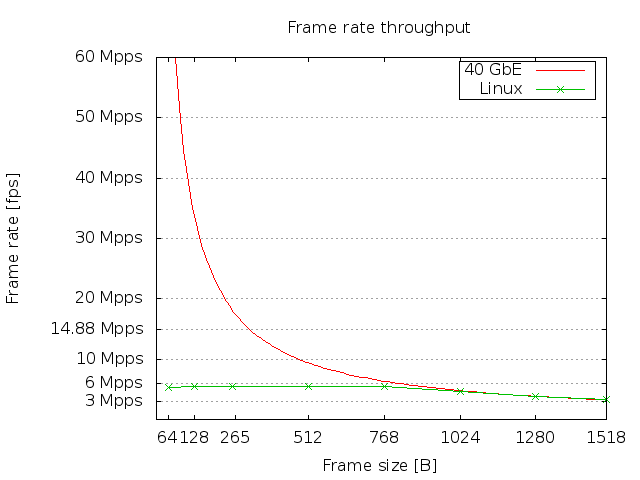
\includegraphics[width=12cm,keepaspectratio]{fig/frames.png}
\end{figure}
\noindent
The system is able to perform forwarding at nearly line rate speed with frames 1024~B and larger.
The following listing shows the actual interrupt mappings obtained from the /proc/interrupts file.
\newpage
%177:       0          0          0          0          0          0          0          0       1655  mlx4-async
\begin{landscape}
\vspace*{\fill}
\begin{lstlisting}
       CPU10      CPU11      CPU12      CPU13      CPU14      CPU15      CPU16      CPU17      CPU18
178:  298717          0          0          0          0          0          0          0          0  enp129s0-0
179:       0     294264          0          0          0          0          0          0          0  enp129s0-1
180:       0          0     291502          0          0          0          0          0          0  enp129s0-2
181:       0          0          0     296514          0          0          0          0          0  enp129s0-3
182:       0          0          0          0     302588          0          0          0          0  enp129s0-4
183:       0          0          0          0          0     294017          0          0          0  enp129s0-5
184:       0          0          0          0          0          0     294314          0          0  enp129s0-6
185:       0          0          0          0          0          0          0     302088          0  enp129s0-7
186:  402863          0          0          0          0          0          0          0          0  enp129s0d1-0
187:       0     411668          0          0          0          0          0          0          0  enp129s0d1-1
188:       0          0     416164          0          0          0          0          0          0  enp129s0d1-2
189:       0          0          0     422023          0          0          0          0          0  enp129s0d1-3
190:       0          0          0          0     421805          0          0          0          0  enp129s0d1-4
191:       0          0          0          0          0     415759          0          0          0  enp129s0d1-5
192:       0          0          0          0          0          0     402918          0          0  enp129s0d1-6
193:       0          0          0          0          0          0          0     413299          0  enp129s0d1-7
\end{lstlisting}
\vspace*{\fill}
\end{landscape}

\noindent
The RX and TX interrupts are spread across 8 CPUs.
The advantage of this mapping against the mapping done by the {\it{irqbalance}} daemon
is that it requires half the CPUs and the IRQ serving should cause fewer cache misses as well.
The listing bellow shows the cache statistics.
\begin{lstlisting}[language=TeX]
 L3MISS: L3 cache misses 
 L2MISS: L2 cache misses (including other core's L2 cache *hits*) 
 L3HIT : L3 cache hit ratio (0.00-1.00)
 L2HIT : L2 cache hit ratio (0.00-1.00)
 L3CLK : ratio of CPU cycles lost due to L3 cache misses (0.00-1.00)
 L2CLK : ratio of CPU cycles lost due to missing L2 cache (0.00-1.00)
 L3OCC : L3 occupancy (in KBytes)
 
 Core (SKT) | L3MISS | L2MISS | L3HIT | L2HIT | L3CLK | L2CLK |  L3OCC
   0    0     5799       33 K    0.82    0.24    0.19    0.18        0
   1    0      122     2488      0.95    0.15    0.03    0.14        0
   2    0      374     3928      0.90    0.19    0.00    0.00        0
   3    0        8      532      0.98    0.15    0.01    0.08       80
   4    0        6      519      0.99    0.16    0.00    0.08        0
   5    0       13      540      0.98    0.13    0.01    0.07        0
   6    0       12      552      0.98    0.14    0.01    0.07        0
   7    0       12      560      0.98    0.14    0.01    0.08      120
   8    0        9      547      0.98    0.13    0.01    0.08        0
   9    0       25      593      0.96    0.13    0.02    0.08        0
  10    1     9527     6014 K    1.00    0.51    0.00    0.14     1080
  11    1     9633     6096 K    1.00    0.52    0.00    0.14     1280
  12    1     9440     6257 K    1.00    0.53    0.00    0.15     1280
  13    1     9349     6069 K    1.00    0.54    0.00    0.14      960
  14    1     9147     6007 K    1.00    0.50    0.00    0.14     1000
  15    1     9270     6043 K    1.00    0.52    0.00    0.15     1160
  16    1     9382     6230 K    1.00    0.52    0.00    0.15     1560
  17    1     9249     6055 K    1.00    0.56    0.00    0.14      920
  18    1     1395     8002      0.83    0.15    0.29    0.29       40
  19    1      198     1129      0.82    0.12    0.13    0.14        0
  20    0      171     1042      0.84    0.08    0.07    0.11       40
  21    0       35     1176      0.97    0.16    0.02    0.17        0
  22    0       24      715      0.97    0.13    0.01    0.11       40
  23    0       18      537      0.97    0.15    0.01    0.09        0
  24    0        5      536      0.99    0.16    0.00    0.09        0
  25    0       11      533      0.98    0.14    0.01    0.08        0
  26    0       15      541      0.97    0.14    0.01    0.08        0
  27    0       11      538      0.98    0.16    0.01    0.09        0
  28    0       14      547      0.97    0.15    0.01    0.09        0
  29    0       46      672      0.93    0.12    0.03    0.10        0
  30    1      557     1200      0.54    0.34    0.03    0.01        0
  31    1      181      612      0.70    0.21    0.26    0.14       40
  32    1      192      604      0.68    0.23    0.25    0.12        0
  33    1      246      634      0.61    0.22    0.31    0.12        0
  34    1      202      622      0.68    0.22    0.28    0.15        0
  35    1      144      599      0.76    0.25    0.20    0.15        0
  36    1      127      620      0.80    0.22    0.17    0.15        0
  37    1      142      619      0.77    0.20    0.21    0.16       40
  38    1      132      685      0.81    0.11    0.13    0.15        0
  39    1      308      921      0.22    0.43    0.38    0.02      360
------------------------------------------------------------------------
 SKT    0     6730       50 K    0.87    0.21    0.03    0.04      280
 SKT    1       85 K     48 M    1.00    0.52    0.00    0.14     9720
------------------------------------------------------------------------
 TOTAL  *       92 K     48 M    1.00    0.52    0.00    0.14     N/A
\end{lstlisting}
As expected, the total cache miss count is lower with the manual IRQ mappings.
\\
The manual mappings are the best IRQ affinity settings in terms of number of CPUs used,
cache use and predictability.

	
	%=========================================================================
% (c) 2014, 2015 Josef Lusticky

% FINAL
\subsection{Measurement 8 - single IPv6 flow}

echo 0 > /proc/sys/net/ipv6/conf/all/disable\_ipv6
echo 1 > /proc/sys/net/ipv6/conf/all/forwarding
again, forwarding on only selected interfaces can be enabled.
ip6tables -F
ip6tables -X
ip6tables -L

ip -6 addr add 1::1/64 dev enp6s0d1
ip -6 addr add 2::1/64 dev enp6s0


%Single IPv6 flow.
%To test the difference between IPv4 and IPv6 routing lookup performance.

\begin{tabular}{ | l | l | l | l | }
\hline
Frame size & \% of link & frame rate \\
\hline
78     &  1.76\% &  0.71~Gb/s & 9~000~000 \\
594    & 11.05\% &  4.42~Gb/s & 9~000~000 \\
1518   & 27.68\% & 11.07~Gb/s & 9~000~000 \\
AMS-IX & 13.69\% &  5.48~Gb/s & 9~000~000 \\
\hline
\end{tabular}

perf top -C 14
\begin{lstlisting}
  11.75%  [kernel]  [k] ip6t_do_table
  10.37%  [kernel]  [k] _raw_spin_lock
   8.43%  [kernel]  [k] fib6_lookup
   4.93%  [kernel]  [k] ip6_forward
   3.66%  [kernel]  [k] fib6_get_table
   3.48%  [kernel]  [k] ip6_rcv_finish
   3.40%  [kernel]  [k] build_skb
   3.26%  [kernel]  [k] __netif_receive_skb_core
   3.01%  [kernel]  [k] mlx4_en_complete_rx_desc
   3.00%  [kernel]  [k] _raw_read_unlock_bh
   2.65%  [kernel]  [k] mlx4_en_process_rx_cq
   2.62%  [kernel]  [k] dst_release
\end{lstlisting}


	%=========================================================================
% (c) 2014, 2015 Josef Lusticky

% FINAL
\subsection{Measurement 9 - 32 IPv6 flows with manual IRQ affinity mappings}
The measurement can be directly compared to Measurement 7.
\\
\\
\begin{tabular}{ | l | l | l | l | }
\hline
Frame size & \% of link & bandwidth & frame rate \\
\hline
78     &  5.88\% &  2.35~Gb/s & 3~000~000 \\
594    & 36.84\% & 14.74~Gb/s & 3~550~000 \\
1518   & 98.50\% & 39.40~Gb/s & 3~202~210 \\
AMS-IX & 54.77\% & 21.91~Gb/s & 3~600~000 \\
\hline
\end{tabular}
\\
\\
The measurement featuring 1518~octet frames was configured to use 98.50\% of the link bandwidth.
The result shows a significant performance drop when routing multiple IPv6 flows.
\\
This performance drop can be investigated by changing the number of UDP flows to 8
and observing the interrupt distribution.
The following listing shows the partial output of the /proc/interrupts file when routing 8 flows.
\begin{lstlisting}
      ... CPU12 CPU13 CPU14 CPU15 CPU16 CPU17 CPU18 ...
 178: ...     0     0     0     0     0     0     0 ... enp129s0d1-0
 179: ...     0     0     0     0     0     0     0 ... enp129s0d1-1
 180: ...     0     0     0     0     0     0     0 ... enp129s0d1-2
 181: ...     0 32513     0     0     0     0     0 ... enp129s0d1-3
 182: ...     0     0     0     0     0     0     0 ... enp129s0d1-4
 183: ...     0     0     0     0     0     0     0 ... enp129s0d1-5
 184: ...     0     0     0     0     0     0     0 ... enp129s0d1-6
 185: ...     0     0     0     0     0 33543     0 ... enp129s0d1-7
 186: ...     0     0     0     0     0     0     0 ... enp129s0-0
 187: ...     0     0     0     0     0     0     0 ... enp129s0-1
 188: ...     0     0     0     0     0     0     0 ... enp129s0-2
 189: ...     0 19384     0     0     0     0     0 ... enp129s0-3
 190: ...     0     0     0     0     0     0     0 ... enp129s0-4
 191: ...     0     0     0     0     0     0     0 ... enp129s0-5
 192: ...     0     0     0     0     0     0     0 ... enp129s0-6
 193: ...     0     0     0     0     0 19576     0 ... enp129s0-7
\end{lstlisting}
In contrast to IPv4, the RSS does not distribute IPv6 packets uniformly.
As a result of this, the routing performance of IPv6 protocol is lower than in case of IPv4.
The traffic is also not distributed uniformly when routing 32 flows,
however, this issue cannot be detected from reading the /proc/interrupts file due to
interrupt mitigation mechanism used by NAPI, as described in subsection~\ref{sub:linux-ingress-napi}.


\section{Upstream mainline kernel 4.0.2}
The following measurements use the upstream Linux kernel downloaded form elrepo, as described in~\ref{sec:analysis-software}.
This is the latest upstream kernel version as of 6th May 2015.
%This allows to use up to 16 queues with RSS.
%The Hyper-Threading must be enabled in order to have at least 16 cores.
%TODO 16 front + HT

	%=========================================================================
% (c) 2014, 2015 Josef Lusticky

%FINAL
\subsection{1 IPv4 flow}
\begin{tabular}{ | l | l | l | l | }
\hline
Frame size & \% of link & bandwidth & frame rate \\
\hline
AMS-IX & 15.22\% &  6.09~Gb/s & 1~000~000 \\
\hline
\end{tabular}
\\
\\
Routing performance of the Linux kernel version 4.0.2 on a single core is the same as the CentOS~7 distribution kernel 3.10.0-123.


\begin{lstlisting}
perf top -C 10
  11.25%  [kernel]            [k] _raw_spin_lock
   9.69%  [kernel]            [k] fib_table_lookup
   5.58%  [kernel]            [k] mlx4_en_xmit
   4.87%  [kernel]            [k] __memcpy
   4.65%  [kernel]            [k] mlx4_en_process_rx_cq
   2.98%  [kernel]            [k] put_compound_page
   2.73%  [kernel]            [k] __netif_receive_skb_core
   2.64%  [kernel]            [k] mlx4_en_poll_tx_cq
   2.43%  [kernel]            [k] ip_route_input_noref
   2.15%  [kernel]            [k] ip_rcv

\end{lstlisting}
FIB table lookup and locking take most of the time,
which is the same result as in case of the CentOS~7 distribution kernel.

	
	%=========================================================================
% (c) 2014, 2015 Josef Lusticky

% FINAL
\subsection{Single IPv6 flow}
\begin{tabular}{ | l | l | l | l | }
\hline
Frame size & \% of link & bandwidth & frame rate \\
\hline
78     &  1.67\% &  0.67~Gb/s & 850~000 \\
594    & 10.44\% &  4.18~Gb/s & 850~000 \\
1518   & 26.15\% & 10.46~Gb/s & 850~000 \\
AMS-IX & 12.93\% &  5.17~Gb/s & 850~000 \\
\hline
\end{tabular}

Kernel profiling:
\begin{lstlisting}
   9.43%  [kernel]  [k] _raw_spin_lock
   6.29%  [kernel]  [k] fib6_lookup_1
   5.49%  [kernel]  [k] mlx4_en_process_rx_cq
   4.12%  [kernel]  [k] mlx4_en_xmit
   3.62%  [kernel]  [k] memcpy
   3.09%  [kernel]  [k] mlx4_en_poll_tx_cq
   3.06%  [kernel]  [k] ip6_pol_route.isra.44
   2.84%  [kernel]  [k] irq_entries_start
   2.22%  [kernel]  [k] dst_release
   2.10%  [kernel]  [k] __netif_receive_skb_core
   2.08%  [kernel]  [k] __local_bh_enable_ip
   1.81%  [kernel]  [k] build_skb
   1.71%  [kernel]  [k] ip6_forward
   1.69%  [kernel]  [k] ipv6_rcv
\end{lstlisting}


	%=========================================================================
% (c) 2014, 2015 Josef Lusticky

% FINAL
\subsection{32 IPv4 flows on 16 queues}
The measurement uses the {\it{ethtool}} utility to configure the Mellanox ConnectX-3 EN adapter to use
16 receive queues per each port.
The network adapter supports up to 16 receive queues per port with RSS,
as described in section~\ref{sec:analysis-hardware}.
\begin{lstlisting}
ethtool -L enp129s0 rx 16
ethtool -L enp129s0d1 rx 16
\end{lstlisting}
The following table shows the result.
\\
\\
\begin{tabular}{ | l | l | l | l | }
\hline
Frame size & \% of link & bandwidth & frame rate \\
\hline
AMS-IX & 81.40\% & 32.56~Gb/s & 5~350~000 \\
\hline
\end{tabular}
\\
\\
Although the networking code runs on 16 logical CPUs simultaneously,
the performance is lower than in case of using 8 queues only.
This may be caused by the overhead of the Hyper-Threading technology.


	%=========================================================================
% (c) 2014, 2015 Josef Lusticky

% FINAL
\subsection{Single IPv6 flow}
The measurement can be directly compared to Measurement 8.
\\
\\
\begin{tabular}{ | l | l | l | l | }
\hline
Frame size & \% of link & bandwidth & frame rate \\
\hline
AMS-IX & 13.69\% &  5.48~Gb/s & 900~000 \\
\hline
\end{tabular}
\\
\\
The single flow routing performance is the same as in case of the CentOS~7 distribution kernel.
The following listing shows the output of the {\it{perf}} tool.
\begin{lstlisting}
perf top -C 10
   9.43%  [kernel]  [k] _raw_spin_lock
   6.29%  [kernel]  [k] fib6_lookup_1
   5.49%  [kernel]  [k] mlx4_en_process_rx_cq
   4.12%  [kernel]  [k] mlx4_en_xmit
   3.62%  [kernel]  [k] memcpy
   3.09%  [kernel]  [k] mlx4_en_poll_tx_cq
   3.06%  [kernel]  [k] ip6_pol_route.isra.44
   2.84%  [kernel]  [k] irq_entries_start
   2.22%  [kernel]  [k] dst_release
   2.10%  [kernel]  [k] __netif_receive_skb_core
   2.08%  [kernel]  [k] __local_bh_enable_ip
   1.81%  [kernel]  [k] build_skb
   1.71%  [kernel]  [k] ip6_forward
   1.69%  [kernel]  [k] ipv6_rcv
\end{lstlisting}


	%=========================================================================
% (c) 2014, 2015 Josef Lusticky

\subsection{32 IPv6 flows}
The measurement can be directly compared to Measurement 9.
\\
\\
\begin{tabular}{ | l | l | l | l | }
\hline
Frame size & \% of link & bandwidth & frame rate \\
\hline
AMS-IX & 54.77\% & 21.91~Gb/s & 3~600~000 \\
\hline
\end{tabular}
\\
\\
As in Measurement~9, the low performance is caused by the RSS distribution done by the network adapter.


\section{Settings influence}
There are various system settings, which can impact the routing performance of the GNU/Linux-based system.
The influence of some the most interesting settings is demonstrated by the following measurements.

	%=========================================================================
% (c) 2014, 2015 Josef Lusticky

% FINAL
\subsection{Disabled Hyper-Threading}
Routing of a single IPv4 flow was tested with the Hyper-Threading technology disabled.
\\
\\
\begin{tabular}{ | l | l | l | l | }
\hline
Frame size & \% of link & bandwidth & frame rate \\
\hline
64     &  1.93\% &  0.77~Gb/s & 1~150~000 \\
594    & 14.12\% &  5.65~Gb/s & 1~150~000 \\
1518   & 35.37\% & 14.15~Gb/s & 1~150~000 \\
AMS-IX & 17.50\% &  7.00~Gb/s & 1~150~000 \\
\hline
\end{tabular}
\\
\\
A single core routing performance increased by 15\% with disabled Hyper-Threading.
\\
Routing of 32 IPv4 flows with manual IRQ affinity mappings was tested to investiage
how is the routing performance influenced when the networking code runs
on multiple cores with Hyper-Threading disabled.
\\
\\
\begin{tabular}{ | l | l | l | l | }
\hline
Frame size & \% of link & bandwidth & frame rate \\
\hline
64     &  9.07\% &  3.63~Gb/s & 5~400~000 \\
594    & 68.77\% & 27.51~Gb/s & 5~600~000 \\
1518   & 98.50\% & 39.40~Gb/s & 3~202~210 \\
AMS-IX & 89.77\% & 35.91~Gb/s & 5~900~000 \\
\hline
\end{tabular}
\\
\\
Disabled Hyper-Threading provides only 2\% performance increase when routing the AMS-IX traffic on multiple cores.
The logical cores which are not utilised do not decrease performance significantly.
Hyper-Threading is highly optimised on Intel Xeon E5-2660 v3.


	%=========================================================================
% (c) 2014, 2015 Josef Lusticky

%FINAL
\subsection{Netdev\_budget}
The measurement increases the {\it{netdev\_budget}} NAPI parameter from its default 300 to 3~000.
The parameter is described in section~\ref{sec:linux-ingress}.
The {\it{netdev\_budget}} can be configured using {\it{procfs}}
\begin{lstlisting}
echo 3000 > /proc/sys/net/core/netdev_budget
\end{lstlisting}

\begin{tabular}{ | l | l | l | l | }
\hline
Frame size & \% of link & bandwidth & frame rate \\
\hline
AMS-IX & 88.25\% & 35.30~Gb/s & 5~800~000 \\
\hline
\end{tabular}
\\
\\
Increasing the {\it{netdev\_budget}} has no influence on routing performance,
which means that the raise softirq mechanism is highly optimised.


	%=========================================================================
% (c) 2014, 2015 Josef Lusticky

%FINAL
\subsection{Reverse path filter}
The measurement features Reverse path filter enabled, which is described in subsection~\ref{sub:analysis-settings-procfs}.
The rp\_filter can be enabled via {\it{procfs}}.
\begin{lstlisting}[language=TeX]
echo 1 | tee /proc/sys/net/ipv4/conf/*/rp_filter
\end{lstlisting}

\begin{tabular}{ | l | l | l | l | }
\hline
Frame size & \% of link & bandwidth & frame rate \\
\hline
AMS-IX & 55.54\% & 22.21~Gb/s & 3~650~000 \\
\hline
\end{tabular}
\\
\\
The rp\_filter introduces a significant performance drop of about 37\%.
The following listing shows the output of the {\it{perf}} utility.
\begin{lstlisting}
perf top -C 10
  39.88%  [kernel]  [k] fib_table_lookup
   8.35%  [kernel]  [k] check_leaf.isra.7
   6.43%  [kernel]  [k] _raw_spin_lock
   2.94%  [kernel]  [k] mlx4_en_xmit
   2.40%  [kernel]  [k] memcpy
   2.32%  [kernel]  [k] __netif_receive_skb_core
   2.18%  [kernel]  [k] mlx4_en_process_rx_cq
   2.14%  [kernel]  [k] fib_validate_source
   1.40%  [kernel]  [k] ip_route_input_noref
\end{lstlisting}
The {\it{fib\_table\_lookup}} is performed twice for each packet
and it is therefore taking much more of the CPU time.
There is also new {\it{fib\_validate\_source}} function, which calls
the actual {\it{fib\_table\_lookup}}.

In bidirectional routing with Reverse path filter enabled,
it may be worth changing the default RSS hash key to a symmetric one.
The RSS hash key is a taken as input by the Toeplitz hash function, as described in section~\ref{sec:linux-scaling}.
A symmetric RSS key would lead to processing both directions of the same flow on the same CPU,
therefore the result of the {\it{fib\_table\_lookup}} could be fetched from the CPU's cache~\cite{symetric-rss}.


	%=========================================================================
% (c) 2014, 2015 Josef Lusticky

%FINAL
\subsection{SELinux}
The measurement features enabled SELinux in Enforcing mode, which can be set in the {\it{/etc/sysconfig/selinux}} file.
\\
\\
\begin{tabular}{ | l | l | l | l | }
\hline
Frame size & \% of link & bandwidth & frame rate \\
\hline
AMS-IX & 80.64\% & 32.26~Gb/s & 5~300~000 \\
\hline
\end{tabular}
\\
\\
SELinux negatively impacts the routing performance by approx.~8.6\%.


	%=========================================================================
% (c) 2014, 2015 Josef Lusticky

\subsection{Firewall}
The measurement features enabled Netfilter and 10~000 filtering rules inserted.
The following commands were used to setup the measurement.
\begin{lstlisting}[language=TeX]
systemctl start firewalld
iptables -F
for i in `seq 10001 20000`; do iptables -A INPUT -p udp --dport $i -j DROP; done
\end{lstlisting}
The {\it{firewalld}} loads Netfilter modules automatically.
\begin{lstlisting}
lsmod | grep nf
nf_conntrack_ipv6      18738  5 
nf_defrag_ipv6         34651  1 nf_conntrack_ipv6
nf_nat_ipv6            13279  1 ip6table_nat
nf_conntrack_ipv4      14862  4 
nf_defrag_ipv4         12729  1 nf_conntrack_ipv4
nf_nat_ipv4            13263  1 iptable_nat
nf_nat                 21798  4 nf_nat_ipv4,nf_nat_ipv6,ip6table_nat,iptable_nat
nf_conntrack          101024  8 nf_nat,nf_nat_ipv4,nf_nat_ipv6,xt_conntrack,ip6table_nat,iptable_nat,nf_conntrack_ipv4,nf_conntrack_ipv6
\end{lstlisting}
The following table shows the results.
\\
\\
\begin{tabular}{ | l | l | l | l | }
\hline
Frame size & \% of link & bandwidth & frame rate \\
\hline
AMS-IX & 88.25\% & 35.30~Gb/s & 5~800~000 \\
\hline
\end{tabular}
\\
\\
The table above shows that 10~000 filtering rules have no impact on throughput.
The following listing shows the output of the {\it{perf}} utility.
\begin{lstlisting}
perf top -C 10
  16.37%  [kernel]  [k] fib_table_lookup
  11.48%  [kernel]  [k] _raw_spin_lock
   6.20%  [kernel]  [k] mlx4_en_process_rx_cq
   5.33%  [kernel]  [k] memcpy
   3.86%  [kernel]  [k] kmem_cache_alloc
   2.90%  [kernel]  [k] check_leaf.isra.7
   2.89%  [kernel]  [k] ipt_do_table
   2.57%  [kernel]  [k] mlx4_en_xmit
   2.42%  [kernel]  [k] mlx4_en_alloc_frags
\end{lstlisting}
The {\it{ipt\_do\_table}} function is responsible for the actual filtering.


	%=========================================================================
% (c) 2014, 2015 Josef Lusticky

\subsection{NAT}
The measurement features a simple Network Address Translation using Netfilter's {\it{MASQUERADE}},
which was configured using {\it{iptables}}.
\begin{lstlisting}
iptables -t nat -A POSTROUTING -o enp129s0 -j MASQUERADE

lsmod | grep nf
  nf_conntrack_ipv4      14862  1 
  nf_defrag_ipv4         12729  1 nf_conntrack_ipv4
  nf_nat_ipv4            13263  1 iptable_nat
  nf_nat                 21798  3 ipt_MASQUERADE,nf_nat_ipv4,iptable_nat
  nf_conntrack          101024  5 ipt_MASQUERADE,nf_nat,nf_nat_ipv4,iptable_nat,nf_conntrack_ipv4
\end{lstlisting}
The following table shows the results.
\\
\\
\begin{tabular}{ | l | l | l | l | }
\hline
Frame size & \% of link & bandwidth & frame rate \\
\hline
AMS-IX & 65.43\% & 26.17~Gb/s & 4~300~000 \\
\hline
\end{tabular}
\\
\\
The performance decreased by approx.~25\% when performing Network Address Translation using {\it{MASQUERADE}}.
Additionally, Netfilter provides other types of Network Address Translation such as {\it{SNAT}} or {\it{SAME}},
however, their description and performance comparison are outside the scope of this thesis.
The following listing shows the output of the {\it{perf}} tool.
\begin{lstlisting}
perf top -C 10
  12.71%  [kernel]  [k] fib_table_lookup
  10.84%  [kernel]  [k] _raw_spin_lock
   6.05%  [kernel]  [k] memcpy
   5.13%  [kernel]  [k] nf_xfrm_me_harder
   4.19%  [kernel]  [k] mlx4_en_process_rx_cq
   2.71%  [kernel]  [k] mlx4_en_xmit
   2.43%  [kernel]  [k] ip_route_input_noref
   2.14%  [kernel]  [k] nf_iterate
   2.07%  [kernel]  [k] check_leaf.isra.7
   2.02%  [kernel]  [k] __netif_receive_skb_core
\end{lstlisting}
The {\it{nf\_xfrm\_me\_harder}} function is responsible for the actual address translation.


\section{BGP routes}

	%=========================================================================
% (c) 2014, 2015 Josef Lusticky

The following measurement is perfomed with the Internet routes obtained from RIPE's BGP data.
The data contains 538~738 routes at the time of writing.
The complete setup of loading the routes into the kernel's FIB is described in appendix~\ref{app:bgp}.
The FIB statistics are exported via the {\it{/proc/net/fib\_triestat}} file, as described in
subsection~\ref{sub:analysis-metodology-collection}.
The following listing shows the content of the file after loading the Internet routes to the kernel's FIB.
\begin{lstlisting}
Basic info: size of leaf: 40 bytes, size of tnode: 40 bytes.
Main:
	Aver depth:     2.43
	Max depth:      8
	Leaves:         503308
	Prefixes:       538739
	Internal nodes: 114429
	  1: 58727  2: 26171  3: 14805  4: 7315  5: 4240  6: 2103  7: 1065  8: 2  17: 1
	Pointers: 995794
Null ptrs: 378058
Total size: 61373  kB

Counters:
---------
gets = 14129134
backtracks = 1913823
semantic match passed = 15973885
semantic match miss = 0
null node hit= 1360956
skipped node resize = 0

Local:
	Aver depth:     3.08
	Max depth:      4
	Leaves:         12
	Prefixes:       13
	Internal nodes: 7
	  1: 6  3: 1
	Pointers: 20
Null ptrs: 2
Total size: 2  kB

Counters:
---------
gets = 13959019
backtracks = 15201204
semantic match passed = 103193
semantic match miss = 0
null node hit= 8238092
skipped node resize = 0
\end{lstlisting}

\begin{tabular}{ | l | l | l | l | }
\hline
Frame size & \% of link & bandwidth & frame rate \\
\hline
AMS-IX & 77.60\% &  30.95~Gb/s & 5~100~000 \\
\hline
\end{tabular}

\begin{lstlisting}
 L3MISS: L3 cache misses 
 L2MISS: L2 cache misses (including other core's L2 cache *hits*) 
 L3HIT : L3 cache hit ratio (0.00-1.00)
 L2HIT : L2 cache hit ratio (0.00-1.00)
 L3CLK : ratio of CPU cycles lost due to L3 cache misses (0.00-1.00)
 L2CLK : ratio of CPU cycles lost due to missing L2 cache (0.00-1.00)
 L3OCC : L3 occupancy (in KBytes)

 Core (SKT) | L3MISS | L2MISS | L3HIT | L2HIT | L3CLK | L2CLK |  L3OCC

   0    0     4048       16 K    0.75    0.40    0.18    0.11      360
   1    0      574     3257      0.82    0.17    0.00    0.00      160
   2    0      515     4977      0.90    0.13    0.06    0.10       40
   3    0        5      539      0.99    0.11    0.00    0.12       40
   4    0        5      526      0.99    0.13    0.00    0.11        0
   5    0        5      532      0.99    0.12    0.00    0.10        0
   6    0        4      548      0.99    0.11    0.00    0.09        0
   7    0        4      541      0.99    0.12    0.00    0.09        0
   8    0        6      548      0.99    0.11    0.00    0.08       40
   9    0       21      550      0.96    0.13    0.01    0.07       40
  10    1     1410 K   9962 K    0.86    0.47    0.09    0.14     2480
  11    1     1400 K   9901 K    0.86    0.46    0.09    0.14     2160
  12    1     1396 K   9872 K    0.86    0.46    0.09    0.14     2200
  13    1     1396 K   9897 K    0.86    0.47    0.09    0.14     2000
  14    1     1402 K   9872 K    0.86    0.46    0.09    0.14     2720
  15    1     1395 K   9861 K    0.86    0.49    0.09    0.14     2160
  16    1     1409 K   9827 K    0.86    0.48    0.09    0.14     2200
  17    1     1402 K   9867 K    0.86    0.46    0.09    0.14     2240
  18    1      398      827      0.52    0.07    0.43    0.11        0
  19    1      200      891      0.78    0.07    0.08    0.09        0
  20    0      213      675      0.68    0.09    0.11    0.06        0
  21    0        7      656      0.99    0.09    0.01    0.13        0
  22    0        6      747      0.99    0.07    0.00    0.12       40
  23    0       13      548      0.98    0.12    0.01    0.12        0
  24    0        4      543      0.99    0.14    0.00    0.11       40
  25    0        5      529      0.99    0.13    0.00    0.10       80
  26    0       25      761      0.97    0.09    0.02    0.13        0
  27    0        5      707      0.99    0.09    0.00    0.12        0
  28    0        5      716      0.99    0.09    0.00    0.11        0
  29    0       45      643      0.93    0.11    0.03    0.09        0
  30    1      362      704      0.49    0.22    0.33    0.06       40
  31    1      206      643      0.68    0.21    0.24    0.12        0
  32    1      187      644      0.71    0.18    0.22    0.12        0
  33    1      188      635      0.70    0.38    0.24    0.13        0
  34    1      193      619      0.69    0.20    0.27    0.14        0
  35    1      208      614      0.66    0.11    0.34    0.15       40
  36    1      184      639      0.71    0.21    0.26    0.15        0
  37    1      194      642      0.70    0.19    0.26    0.13        0
  38    1      181      616      0.71    0.09    0.23    0.13        0
  39    1       22 K     29 K    0.24    0.16    0.85    0.06      200
------------------------------------------------------------------------
 SKT    0     5515       35 K    0.84    0.28    0.02    0.03       840
 SKT    1       11 M     79 M    0.86    0.47    0.09    0.14     18440
------------------------------------------------------------------------
 TOTAL  *       11 M     79 M    0.86    0.47    0.09    0.14     N/A
\end{lstlisting}

